\section{Avslut}
\begin{frame}
\frametitle{Innehåll}
\tableofcontents[currentsection]
\end{frame}

\begin{frame}{Vad innebär allt detta?}



\begin{columns}
    \begin{column}{0.6\textwidth}
        \begin{itemize}
			\item Elektronisk röstning är möjligt
			\item Inte riktigt där \emph{än}
			\item Verificatum i norska valet
		\end{itemize}
    \end{column}
	\begin{column}{0.4\textwidth}
    	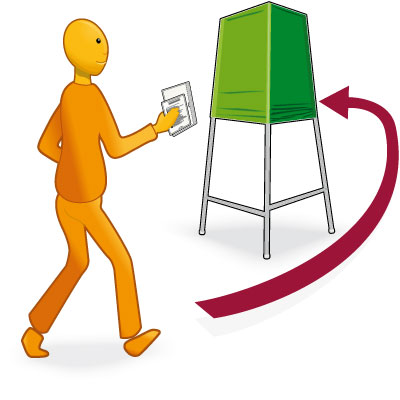
\includegraphics[width=\textwidth]{images/rosta.jpg}
	\end{column}
\end{columns}

\end{frame}

\begin{frame}{Tack för oss! Frågor?}

\begin{columns}
    \begin{column}{0.4\textwidth}
        \begin{itemize}
			\item Tack för att ni lyssnade!
			\item Har ni frågor?
		\end{itemize}
    \end{column}
	\begin{column}{0.6\textwidth}
    	\includegraphics[height=0.7\textheight]{images/interrobang.png}
	\end{column}
\end{columns}

\end{frame}
